\thispagestyle{empty}
\null\vspace{\stretch{2}}
{\centering
	{\bfseries
		{\fontsize{28}{44}\selectfont\MakeTitre{}}\\
		{\fontsize{14}{44}\selectfont\version{}}\par
		{\fontsize{20.74}{22}\selectfont\soustitre}\par
		\vspace{\stretch{1}}
		{\fontsize{12}{36}\selectfont\MakeAuteur}\par
		\vspace{\stretch{1}}
		\begin{figure}[h]%
			\begin{center}%
				\leavevmode%
				\subfigure{%
					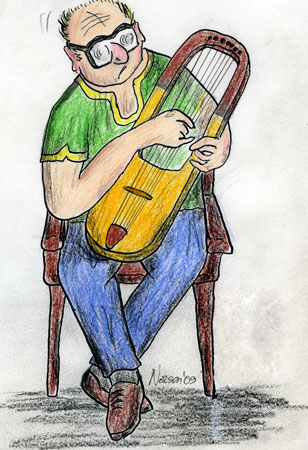
\includegraphics[width=4cm]{main/Logo_Livre.jpg}}%
				\hspace{1cm}%
			\end{center}%
		\end{figure}%
	}\newpage\thispagestyle{empty}
	{\bfseries\fontsize{14}{16}\selectfont{}ÉDITIONS}\par

	{\fontsize{14}{16}\selectfont{}La forêt du grand Méchant Loup\\
														Adresse Non disponible\\
														666 Avenue du Libre }\par
	\vspace{\stretch{3}}
	{\fontsize{12}{14}\selectfont{}Ce livre et l'illustration en couverture sont publiés sous la licence libre\\\textbf{Creative Commons-BY-SA} :\\\url{http://creativecommons.org/licenses/by-sa/2.0/fr}\par}
}
{\setlength{\parskip}{1.5\baselineskip}
	\textbf{BY : Paternité.} Vous devez citer le nom de l'auteur original.\par
	\textbf{SA : Partage des Conditions Initiales à l'Identique.} Si vous modifiez, transformez ou adaptez cette création, vous n'avez le droit de distribuer la création qui en résulte que sous un contrat identique à celui-ci.\\
	En outre, à chaque réutilisation ou distribution, vous devez faire apparaître clairement aux autres les conditions contractuelles de mise à disposition de cette création. Chacune de ces conditions peut être levée si vous obtenez l'autorisation du titulaire des droits.\par
}
\vspace{\stretch{2}}
{\centering\setlength{\parskip}{2\baselineskip}
	In Libro Veritas, \anneedepot{}, ISBN : \isbn\par
	Dépôt légal : \datedepot\par
}
\vspace{\stretch{4}}